%Tex root = LInguaggi.tex

\chapter{Descrivere i linguaggi di programmazione}
Un linguaggio di programmazione è un formalismo artificiale utilizzato per esprimere algoritmi.\\[0.2ex]
Anche se artificiale, è sempre un linguaggio e, quindi, deve essere descritto.

\smallskip
Un linguaggio di programmazione non è altro che come un linguaggio naturale, ma semplificato e non ambiguo.\\[0.2ex]
La descrizione di un linguaggio PL avviene tramite:
\begin{itemize}[label=$\triangleright$, itemsep=\smallskipamount]
    \item \textbf{sintassi} (grammatica): regole di formazione di frasi ben formate (descrive relazione tra segni)
    \item \textbf{semantica}: attribuzione di significato ai simboli della sintassi (costruisce relazione tra segni e significato)
    \item \textbf{pragmatica}: modo in cui le frasi del linguaggio di programmazione vengono usate
    \item \textbf{implementazione}: strumenti per eseguire frasi del linguaggio di programmazione rispettandone la semantica
\end{itemize}

\section{Sintassi}
\begin{mydef}{sintassi}
    Le \textbf{regole sintattiche} del linguaggio specificano quali stringhe di caratteri sono legali nel linguaggio.
\end{mydef}

La terminologia nella linguistica sono:
\begin{itemize}[label=$\circ$, itemsep=\smallskipamount]
    \item \textbf{parola}: sequenza (stringa) di caratteri in un alfabeto
    \item \textbf{frase}: sequenza (ben formata) di parole
    \item \textbf{linguaggio}: insieme di frasi
\end{itemize}

Nell'ambito dei linguaggi di programmazione, gli stessi nomi prendono nomi differenti:
\begin{itemize}[label=$\diamond$, itemsep=\smallskipamount]
    \item \textbf{lessema} (parola): parola (terminale) con significato proprio.
    
    Corrisponde all'\hl{unità sintattica a più basso livello dei PL}.
    \item \textbf{token} (frase): sequenze di simboli non terminali.
    
    Corrispondono agli \hl{elementi delle categorie sintattiche}.
\end{itemize}

\subsection{Descrivere la sintassi}
Abbiamo bisogno di strumenti formali per descrivere parole e frasi ben formate di un linguaggio. che permettono, in modo automatico, di verificare l'appartenenza o meno al linguaggio.

\begin{mydef}{riconoscitore}
    Il \textbf{riconoscitore} è uno strumento (formale) di riconoscimento che legge in input stringhe sull'alfabeto e decide se la stringa appartiene o meno al linguaggio.

    \smallskip
    \textcolor{red}{\textbf{Es}}. automi a stati finiti (analisi sintattica)
    \begin{figure}[H]
        \centering
        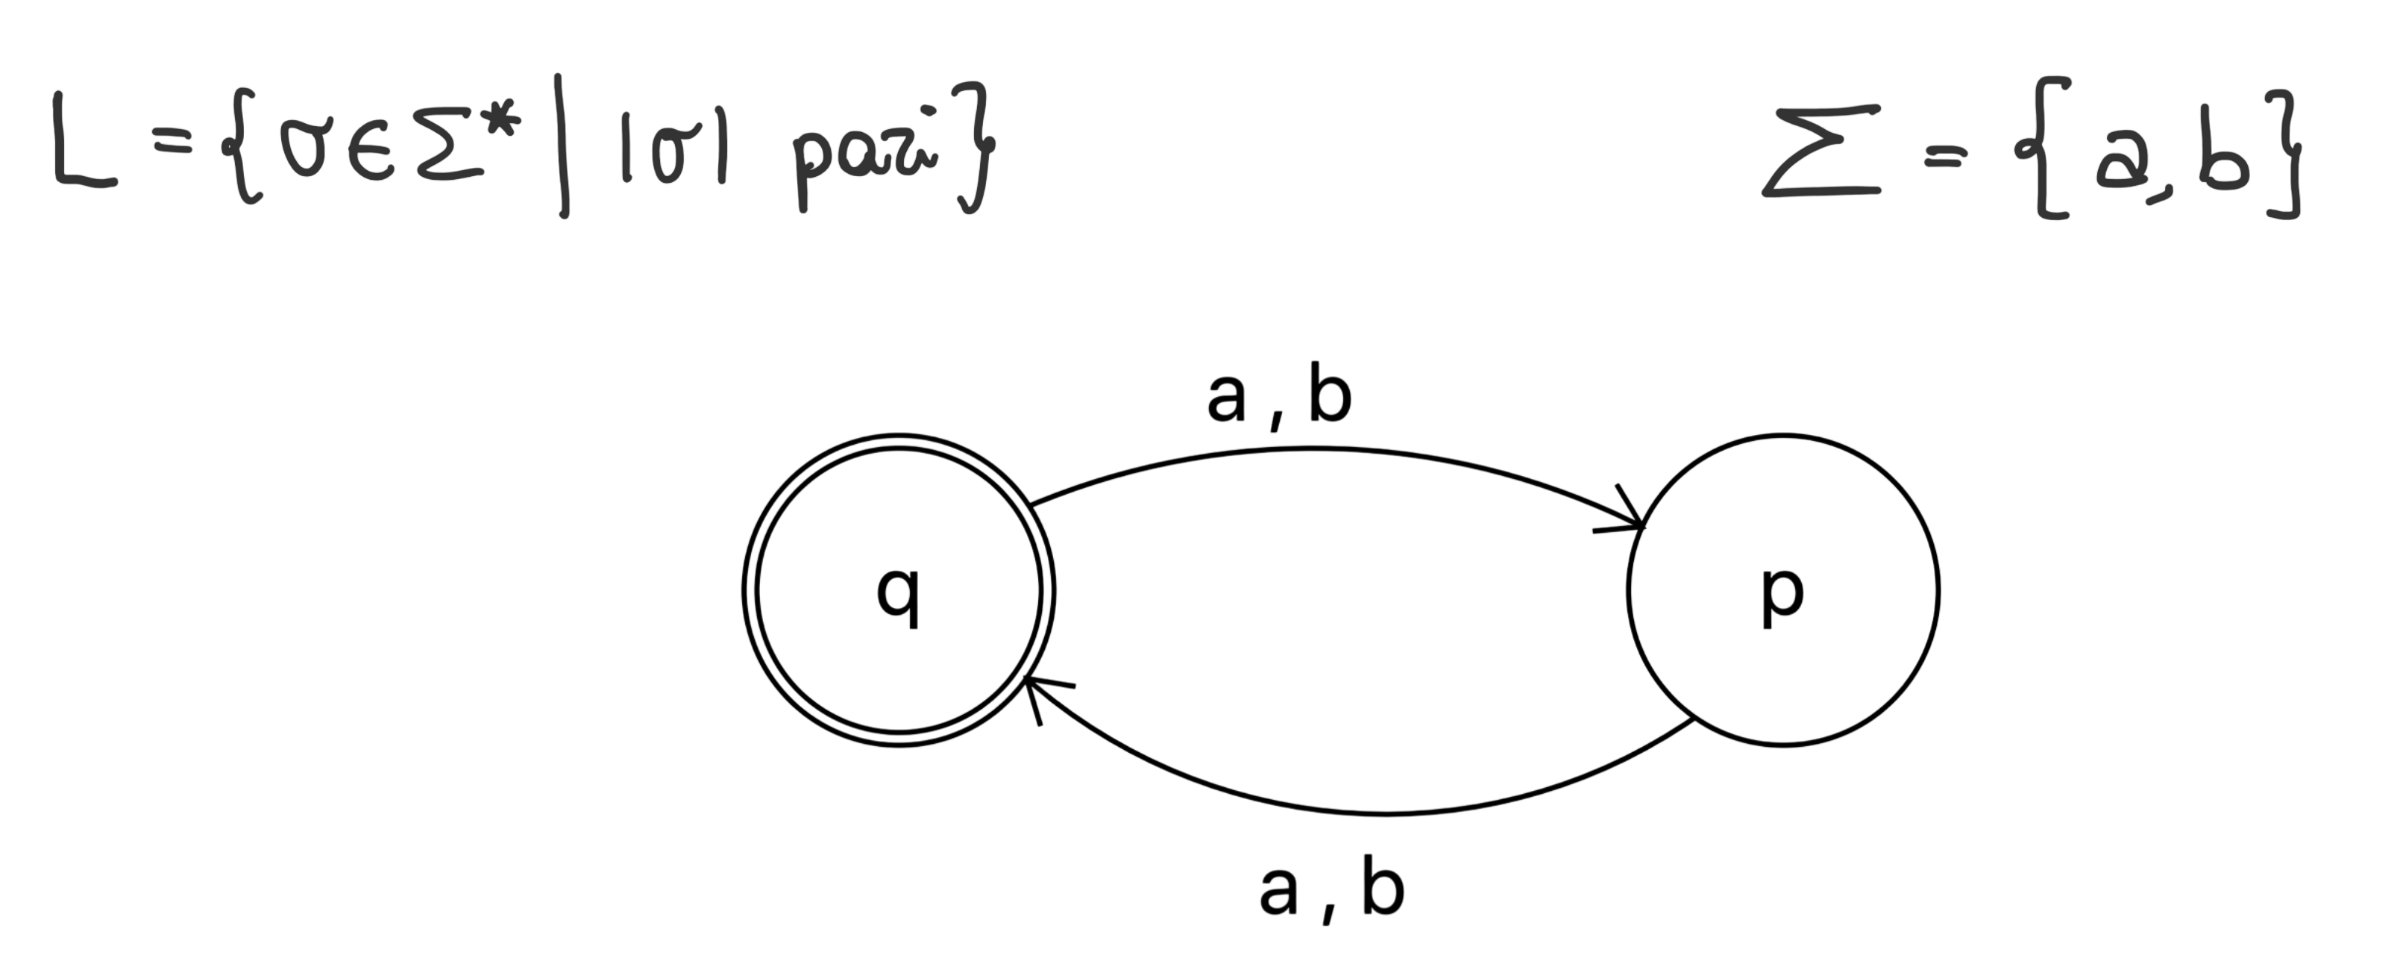
\includegraphics[width=0.5\textwidth]{images/riconoscitore-ASF.png}
         \caption{esempio di automa a stati finiti}
    \end{figure}
\end{mydef}

\begin{mydef}{generatore}
    Il \textbf{generatore} è uno strumento (formale) che genera stringhe di un linguaggio.

    \smallskip
    \textcolor{red}{\textbf{Es}}. grammatiche CF (parser)
    \begin{figure}[H]
        \centering
        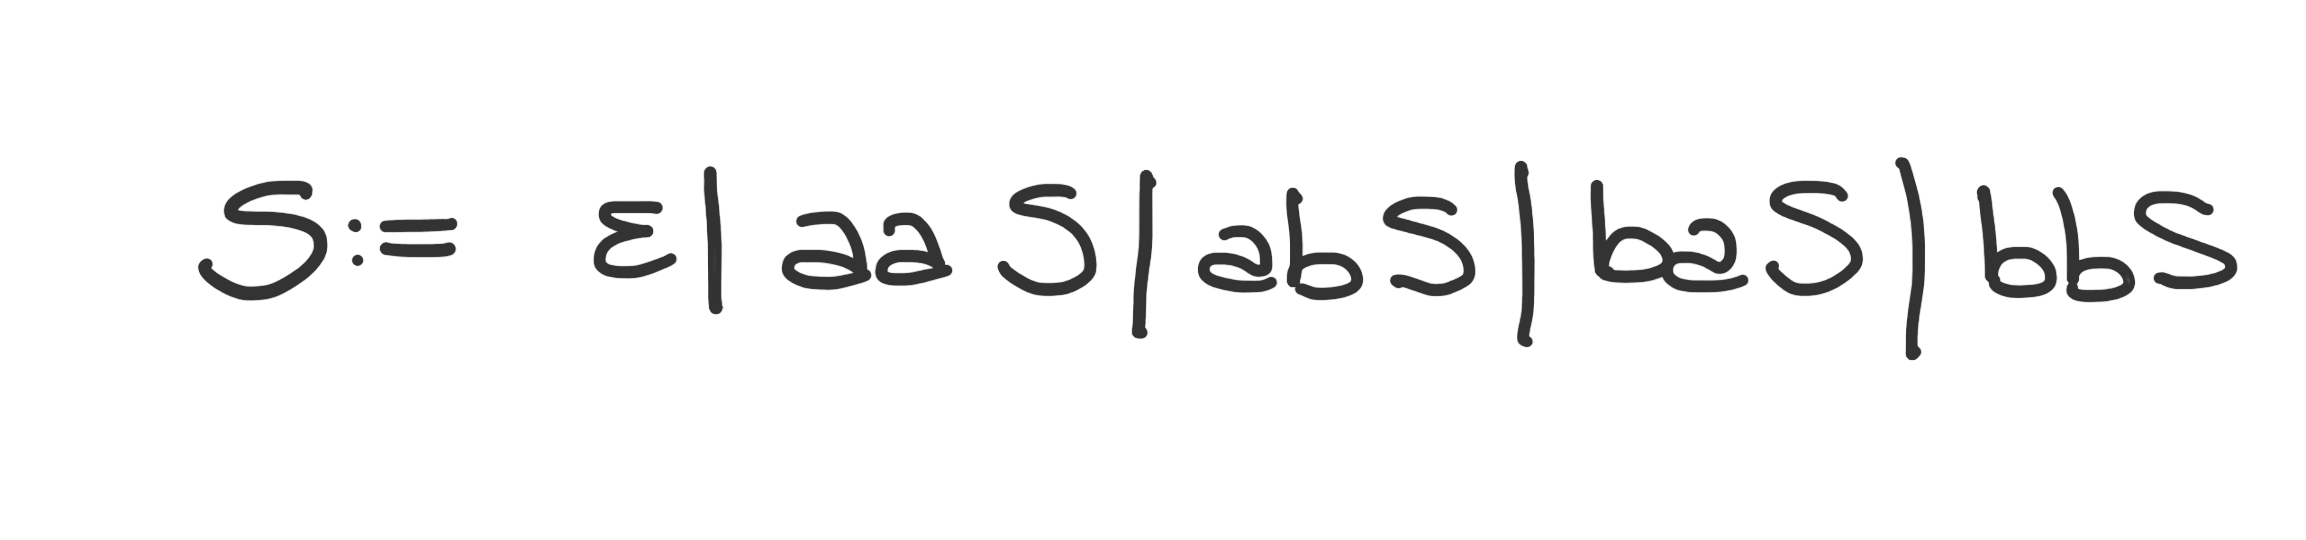
\includegraphics[width=0.5\textwidth]{images/generatore.png}
        \caption{esempio di stringhe generate da un automa a stati finiti}
    \end{figure}
\end{mydef}

\subsection{Grammatiche CF}
La grammatica descrive i modi per combinare parole e formare frasi ed è descritta da:
\begin{itemize}[label=$\triangleright$, itemsep=\smallskipamount]
    \item \textbf{alfabeto}
    \item \textbf{descrizione lessicale}: descrizione delle parole
    \item \textbf{descrizione delle frasi}
\end{itemize}

\esempio{grammatica}{
    \begin{figure}[H]
        \centering
        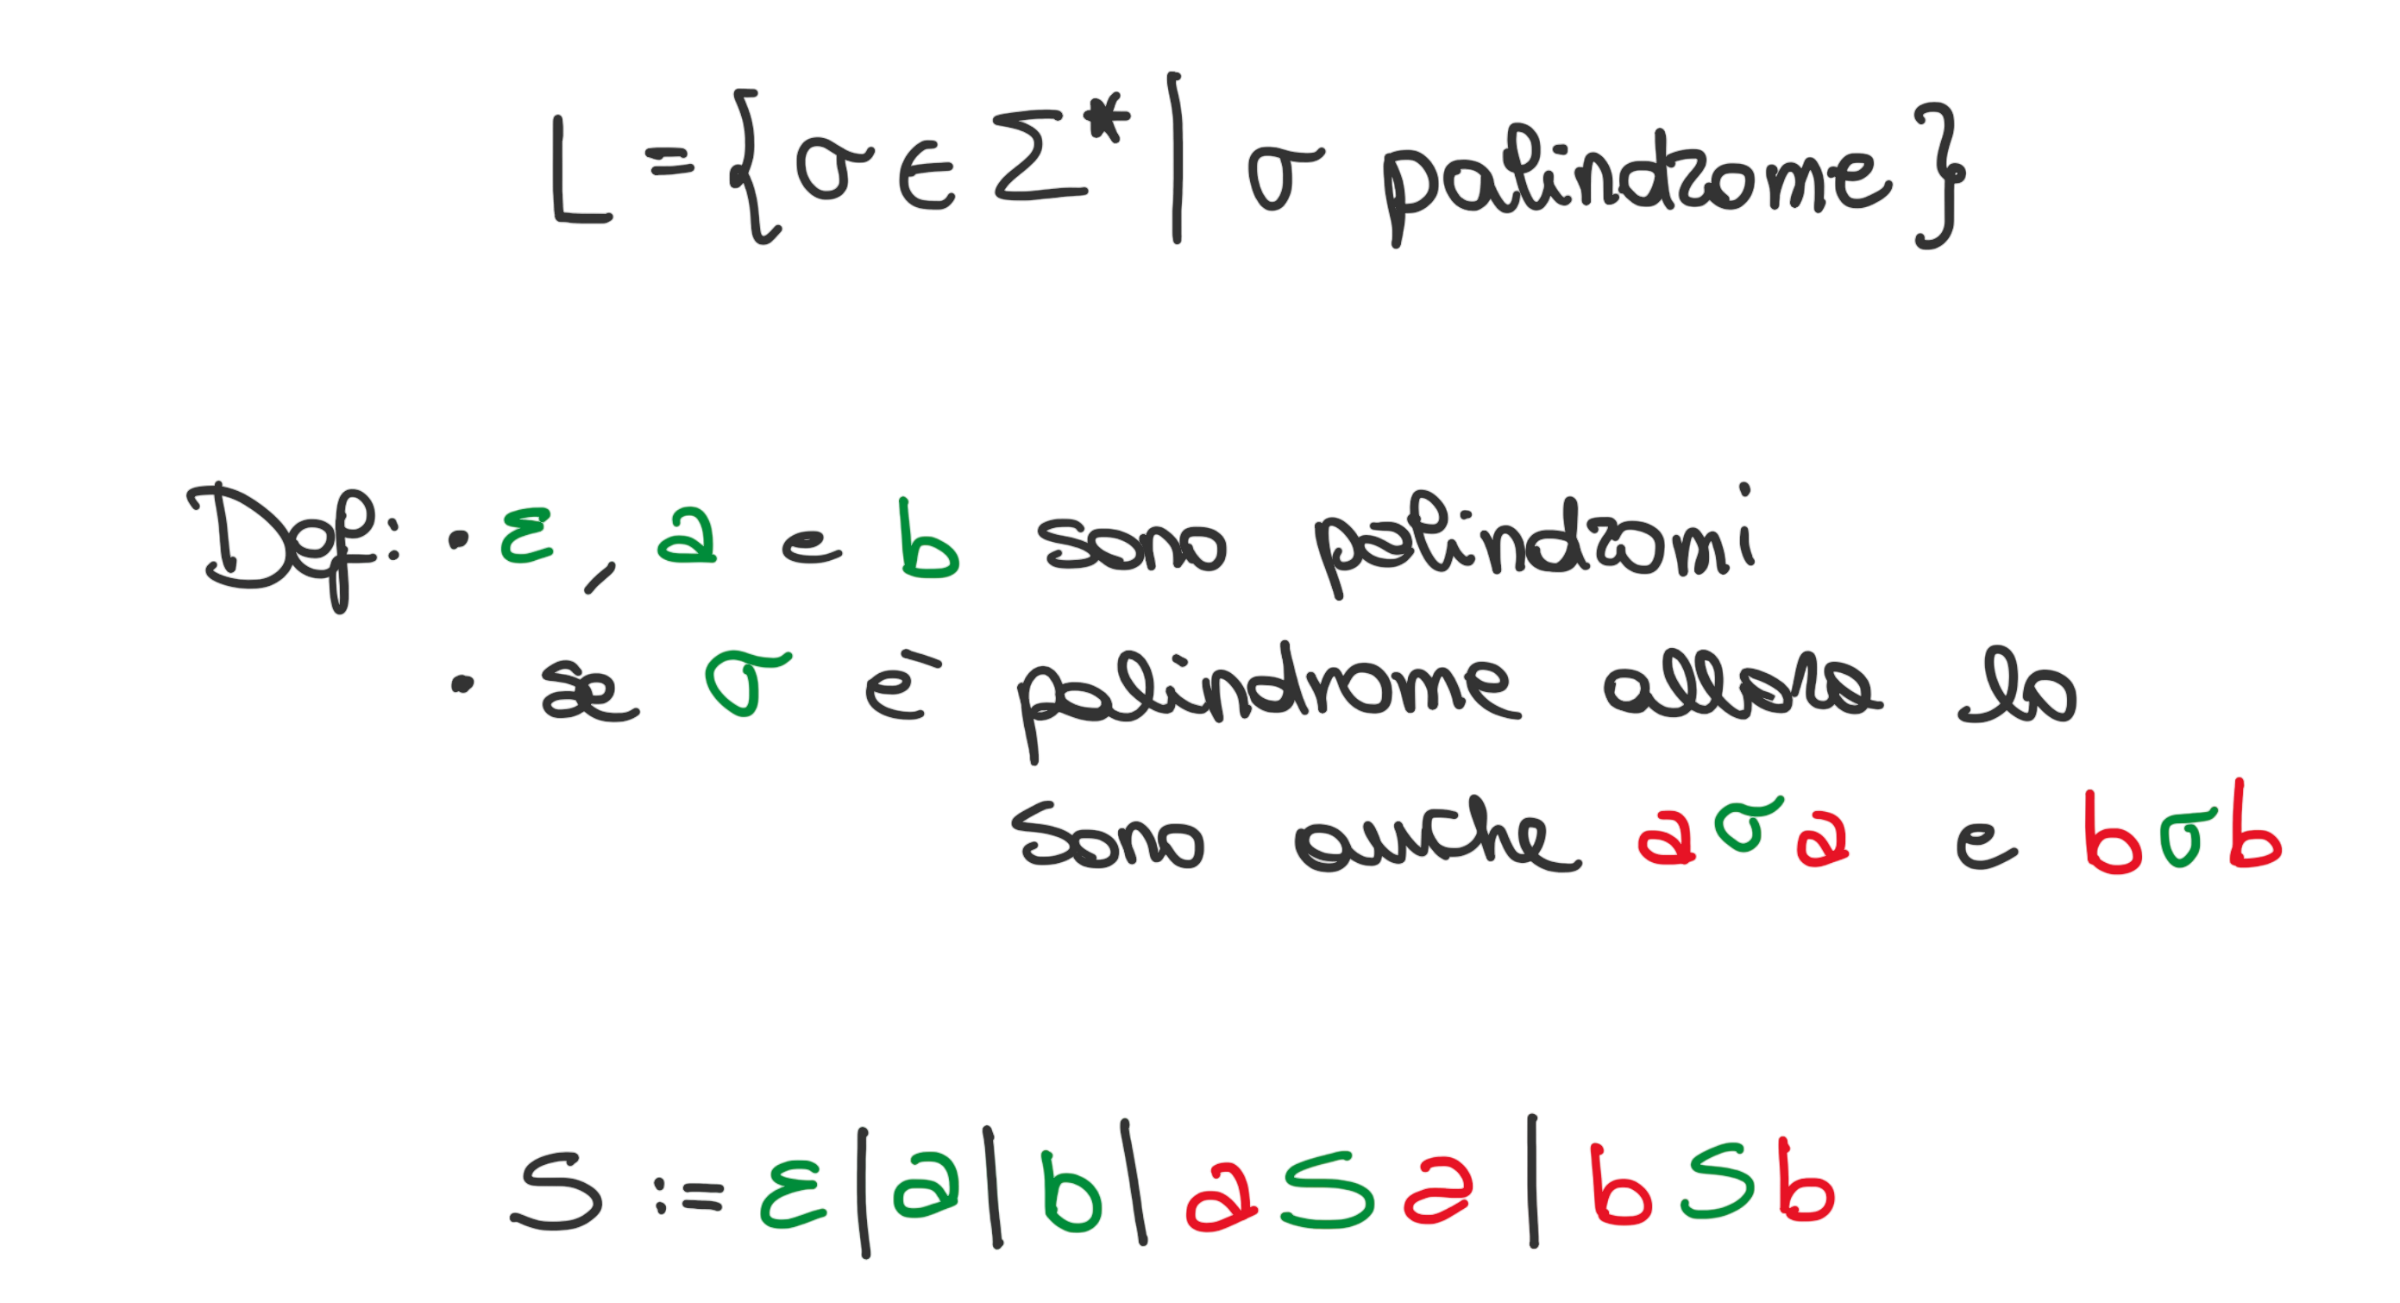
\includegraphics[width=0.8\textwidth]{images/esempio-grammaticaCF.png}
    \end{figure}
}

Per costruire una grammatica abbiamo bisogno di:
\begin{itemize}[label=$\circ$, itemsep=\smallskipamount]
    \item \textbf{vocabolario}
    \item \textbf{regole di composizione}: come combinare le parole (produzioni) per ottenere frasi ben formate
\end{itemize}

\bigskip
Le grammatiche CF permettono di descrivere la sintassi dei linguaggi di programmazione.\\[0.2ex]
Questo gereratore di linguaggi è stato sviluppato da Chomsky per descrivere la sintassi dei linguaggi naturali e permette di definire la classe de linguaggi CF.

\begin{mydef}{grammatica CF}
    Una \textbf{grammatica CF} è una quadrupla
    \[
        \mathrm{G = \langle V, T, P, S \rangle}
    \]

    dove:
    \begin{itemize}[label=$\diamond$, itemsep=\smallskipamount]
        \item \textbf{V}: insieme dei simboli non terminali
        \item \textbf{T}: insieme dei simboli terminali ($V \cup T = \emptyset$)
        \item \textbf{P}: insieme delle produzioni
        \[
            \underbrace{\underbrace{\mathrm{A}}_{\mathrm{\in \ V}} \rightarrow \alpha \in (\mathrm{V \cup T})^*}_{\text{\parbox{8cm}{\textcolor{red}{a un simbolo non terminale A possiamo sostituire (indipendente dal contesto) la sequenza $\alpha$ di simboli terminali e non}}}}
        \]
        \item $\underbrace{\mathbf{S \in V}}_{\text{\parbox{1.5cm}{\textcolor{red}{rappresenta il linguaggio da generare}}}}$: simbolo iniziale
    \end{itemize}
\end{mydef}

Nella grammatica i simboli terminali costituiscono il vocabolario (collezione di parole/token), invece, i simboli non terminali sono le categorie sintattiche (espressioni, comandi, dichiarazioni, ecc.).\\[0.2ex]
Le produzioni sono le regole di formazione/composizione (istruzioni $\dots$ programmi).\\[0.2ex]
Il linguaggio è l'insieme di tutte le frasi (stringhe di simboli terminali) generate a partire dal simbolo inziale $\mathrm{S}$.

\subsubsection{Notazione BNF}
La notazione BNF viene ideata nel 1959 da Bakus per \texttt{Algol60}.\\[0.2ex]
Questa notazione è usata per descrivere grammatiche CF, dove si usano intere parole come simboli terminali, mentre i non terminali sono identificati racchiudendoli tra parentesi angolate \texttt{<>}.\\[0.2ex]
Per le produzioni, invece, viene utilizzato il simbolo \texttt{:=} al posto della freccia \texttt{->}.

\begin{figure}[H]
    \centering
    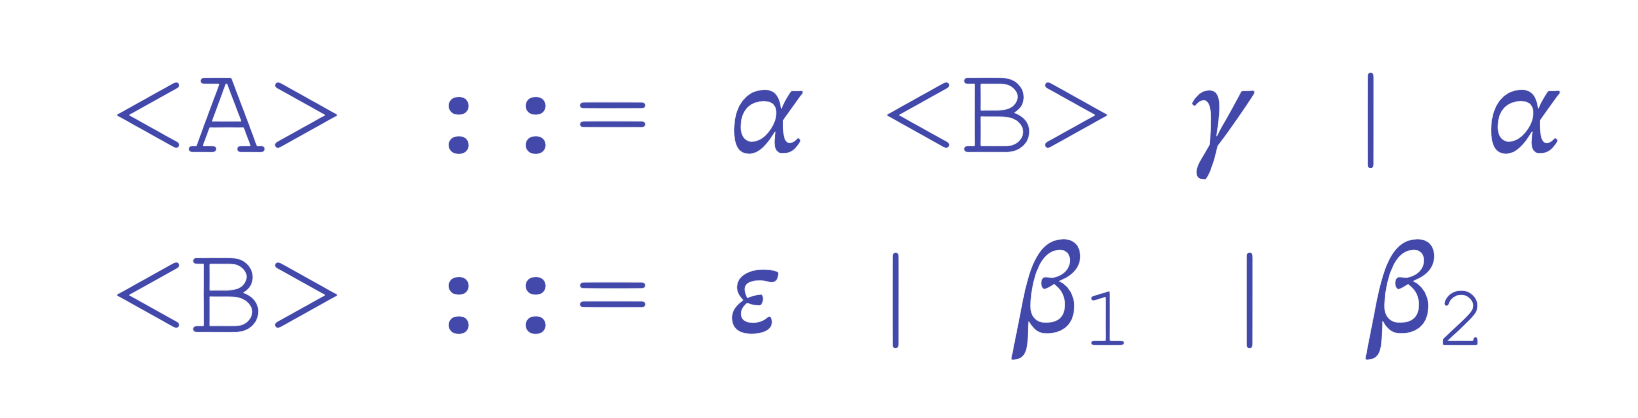
\includegraphics[width=0.5\textwidth]{images/esempio-notazione-BNF.png}
    \caption{esempio di notazione BNF}
\end{figure}

\subsection{Descrivere un semplice linguaggio imperativo}
Un linguaggio può essere descritto anche in modo informalel descrivendo quali caratteristiche deve avere qual è il loro significato:
\begin{itemize}[label=$\triangleright$, itemsep=\smallskipamount]
    \item niente dichiarazioni
    \item solo variabili ed espresisoni booleane
    \item assegnamento e composizione sequenziale
    \item comando condizionale
    \item comando imperativo (loop)
\end{itemize}

Anche i lingauggi di programmazione sono descritti a livelli di astrazione, ognuno descritto da una grammatica.
\begin{figure}[H]
    \centering
    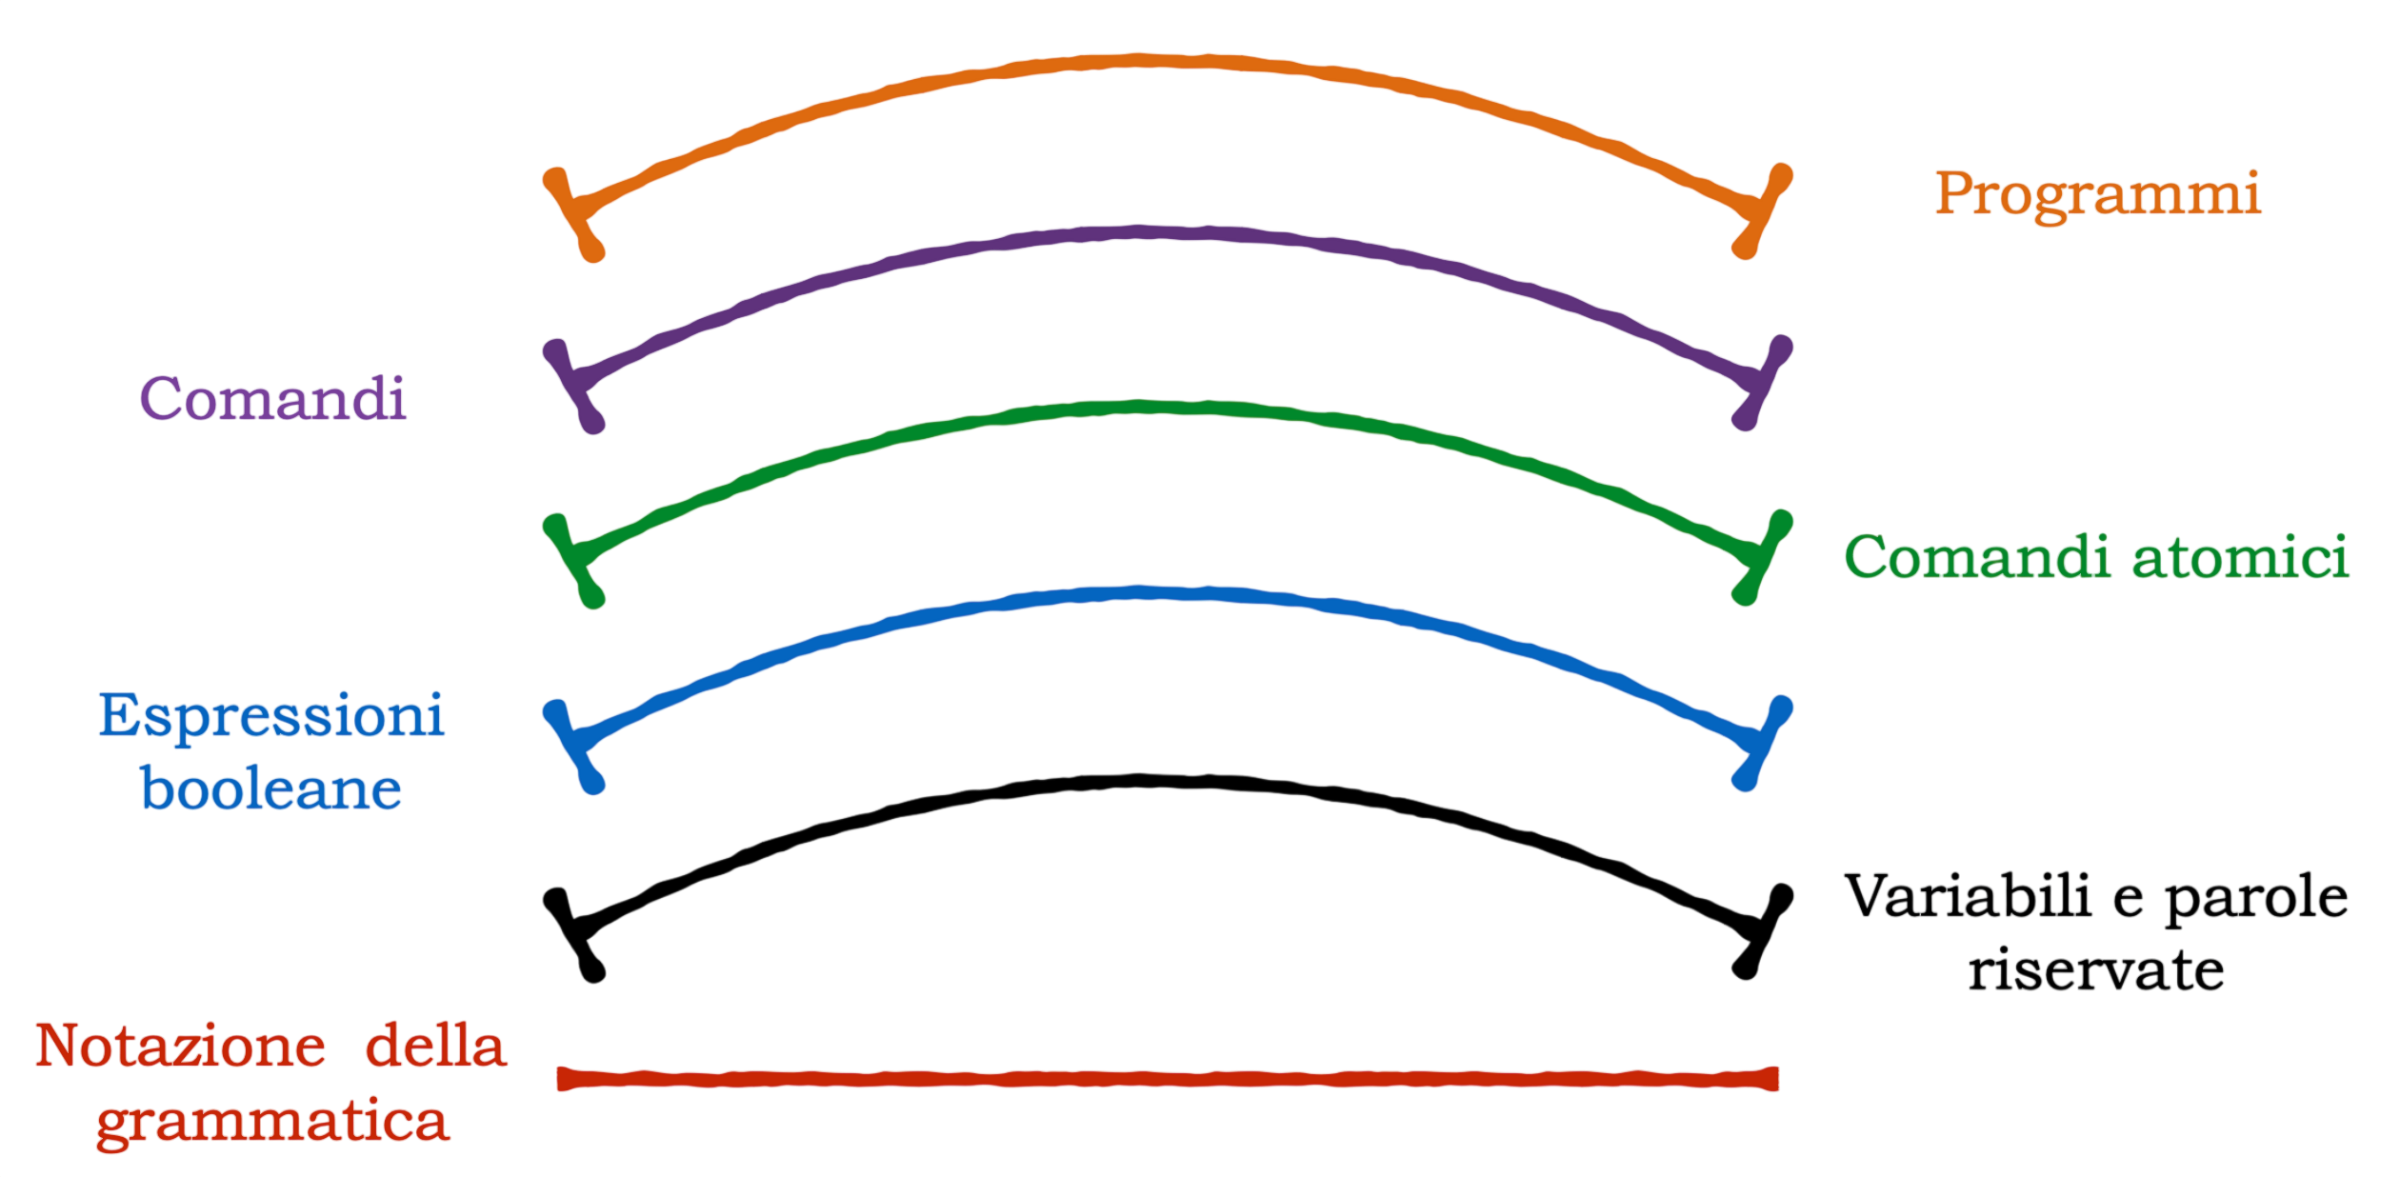
\includegraphics[width=0.6\textwidth]{images/astrazione-PL.png}
    \caption{livelli di astrazione dei PL}
\end{figure}

\begin{bnfcode}{Notazione grammatica}
<bExpr> B -> true | false | v | (not B) | (B and B) | (B or B)

<atomic com>  A -> v := B

<com> C -> A | C ; C | if B then C else C | while B do C

<program> S -> C
\end{bnfcode}

\subsubsection{Analisi semantica}
Esistono dei vincoli che la grammatica CF non può catturare:
\begin{itemize}[label=$\triangleright$, itemsep=\smallskipamount]
    \item \textbf{vincoli contestuali}: dichiarare una variabile prima dell'uso, $\mathrm{n^\circ}$ di parametri di una chiamata
\end{itemize}

Il problema è che non esistono algoritmi per il riconoscimento di stringhe generate, quindi, non ci sono algoritmi per fare il parser di queste stringhe.\\[0.2ex]
Per questo la scelta ricade su una specifica del linguaggio mediante grammatica CF (sintassi) e poi, come parte della semantica (semantica statica) vengono specificati i vincoli contestuali.

\section{Semantica}

\section{Categorie sintattiche}